\documentclass[12pt, aspectratio=169]{beamer}
% \documentclass[12pt, aspectratio=169, handout]{beamer}
% [8pt], [9pt], [10pt], [11pt], [12pt], [14pt], [17pt], [20pt], [bigger], and [small]

% ============================================================
% Shared preamble for 2103304 Automatic Control I (Fall 2026)
% Lectures. Load from each main.tex with: % ============================================================
% Shared preamble for 2103304 Automatic Control I (Fall 2026)
% Lectures. Load from each main.tex with: % ============================================================
% Shared preamble for 2103304 Automatic Control I (Fall 2026)
% Lectures. Load from each main.tex with: \input{../preamble.tex}
% Per-lecture \title/\subtitle/\author/\date/\logo stay in main.tex.
% ============================================================

% Resolve graphics from each lecture's standard subfolders, then shared root.
% Paths are relative to the main.tex being compiled, so this works for any
% lecture that follows the convention and sits one level under Lecture/.
\graphicspath{{./}{./graphic_files/}{./tex_files/}{./matlab_files/}{../shared_graphics/}{../shared_graphics/Logo/}}

\usepackage[utf8]{inputenc}
\usepackage{matlab-prettifier}
% \usepackage{setspace} % line space control (corrupted footnote)

%maths
\usepackage{mathtools}
\usepackage{amsmath}
\usepackage{amssymb}
\usepackage{amsfonts}

%tikzpicture
\usepackage{tikz}
\usepackage{scalerel}
\usepackage{pict2e}
\usepackage{tkz-euclide}
\usetikzlibrary{calc}
\usetikzlibrary{patterns,arrows.meta}
\usetikzlibrary{shadows}
\usetikzlibrary{external}
\usepackage[american,siunitx]{circuitikz} %for drawing circuit

%pgfplots
\usepackage{pgfplots}
\pgfplotsset{compat=newest}
\usepgfplotslibrary{statistics}
\usepgfplotslibrary{fillbetween}
\usepgfplotslibrary{groupplots}

\usepackage{nicefrac}
\usepackage{booktabs}

% video playback in beamer: \movie[externalviewer]{link text}{file.mp4}
\usepackage{multimedia}

% set up chula color theme
\usepackage{xcolor}
\usepackage{colortbl}

% Brand colors
\definecolor{brandred}{HTML}{8B2332}
\definecolor{brandblack}{HTML}{231F20}
\definecolor{brandredME}{HTML}{4C1E29} % Mechanical Engineering dark maroon

% Optional: lighter tints (matching the % shades in your palette)
\definecolor{brandred80}{HTML}{A24F5B}
\definecolor{brandred60}{HTML}{BC8088}
\definecolor{brandred40}{HTML}{D5AFB4}
\definecolor{brandred20}{HTML}{ECD7D9}
\definecolor{brandgray60}{HTML}{6F6D6E}
\definecolor{brandgray30}{HTML}{B7B6B6}

\usetikzlibrary{shapes,arrows}
\usetikzlibrary{shapes.misc}
\usepgfplotslibrary{fillbetween}

% use the colortbl package to define a new column i
\newcolumntype{a}{>{\columncolor{brandred20}}c}

% \usetheme{Copenhagen}
% \usetheme{Berlin}
% \usetheme{Antibes}

\usetheme{Luebeck}
% \usetheme{Madrid}

% \usecolortheme{default}
% \usecolortheme{seahorse}

% use chula color theme
% Structure (titles, headings, etc.)
\setbeamercolor{structure}{fg=brandred}
% Title page
\setbeamercolor{title}{fg=white, bg=brandred}
\setbeamercolor{frametitle}{fg=white, bg=brandred}
% Body text
\setbeamercolor{normal text}{fg=brandblack}
% Blocks
\setbeamercolor{block title}{fg=white, bg=brandred}
\setbeamercolor{block body}{fg=brandblack, bg=brandred20}

% Source - https://tex.stackexchange.com/a/26284
% Posted by percusse
% Retrieved 2026-07-17, License - CC BY-SA 3.0
% \setbeamercolor{postit}{fg=brandblack,bg=brandred20}
% \begin{beamercolorbox}[sep=1em,wd=5cm]{postit}
% Place me somewhere!
% \end{beamercolorbox}


% Bullets / itemize
\setbeamercolor{itemize item}{fg=brandred}
\setbeamercolor{itemize subitem}{fg=brandgray60}

% convert to handout
% \usepackage{pgfpages}
% \pgfpagesuselayout{4 on 1}{a4paper, border shrink=5mm}

\setbeamertemplate{navigation symbols}{} % hide navigation symbol
\setbeamertemplate{page number in head/foot}{\insertframenumber \slash \inserttotalframenumber}

% \setbeamercovered{transparent}
% \setbeamercovered{invisible}

\setbeamertemplate{headline}{} % hide navigation bar at the top

\usepackage{bm}
\usefonttheme[onlymath]{serif}

% spacing in table https://latex-beamer.com/tutorials/beamer-table/#insert-table-beamer
% Change horizontal spacing
\setlength{\tabcolsep}{20pt}
% Change vertical spacing
\renewcommand{\arraystretch}{1.25}
% use the colortbl package to define a new column
\newcolumntype{g}{>{\columncolor{brandgray30}}l}

% Fill-in convention: \fillin{...} renders a gray italic placeholder.
\newcommand{\fillin}[1]{\textcolor{gray}{\textit{[#1]}}}

% Unnumbered footnote (e.g. image credits): \blfootnote{...}
\newcommand\blfootnote[1]{
    \begingroup
    \renewcommand\thefootnote{}\footnote{#1}
    \addtocounter{footnote}{-1}
    \endgroup
}

% Show a section-outline frame at the start of each \section
\AtBeginSection[]
{
  \begin{frame}
    \frametitle{Lecture Outline}
    \tableofcontents[currentsection]
  \end{frame}
}

%------------------------------------------------------------
% Title are set in each lecture's main.tex, not here.
%------------------------------------------------------------

\author[2103304 Automatic Control I (Fall 2026)] % (optional, for multiple authors)
{\textbf{Chawin Ophaswongse, Ph.D.}}

\date[Mech. Eng., Chulalongkorn University] % (optional)
{2103304 Automatic Control I (Fall 2026) \newline \newline Department of Mechanical Engineering \newline Faculty of Engineering, Chulalongkorn University}

\logo{
\includegraphics[height=0.5cm]{Logo CHULA ENG.pdf}}

% Per-lecture \title/\subtitle/\author/\date/\logo stay in main.tex.
% ============================================================

% Resolve graphics from each lecture's standard subfolders, then shared root.
% Paths are relative to the main.tex being compiled, so this works for any
% lecture that follows the convention and sits one level under Lecture/.
\graphicspath{{./}{./graphic_files/}{./tex_files/}{./matlab_files/}{../shared_graphics/}{../shared_graphics/Logo/}}

\usepackage[utf8]{inputenc}
\usepackage{matlab-prettifier}
% \usepackage{setspace} % line space control (corrupted footnote)

%maths
\usepackage{mathtools}
\usepackage{amsmath}
\usepackage{amssymb}
\usepackage{amsfonts}

%tikzpicture
\usepackage{tikz}
\usepackage{scalerel}
\usepackage{pict2e}
\usepackage{tkz-euclide}
\usetikzlibrary{calc}
\usetikzlibrary{patterns,arrows.meta}
\usetikzlibrary{shadows}
\usetikzlibrary{external}
\usepackage[american,siunitx]{circuitikz} %for drawing circuit

%pgfplots
\usepackage{pgfplots}
\pgfplotsset{compat=newest}
\usepgfplotslibrary{statistics}
\usepgfplotslibrary{fillbetween}
\usepgfplotslibrary{groupplots}

\usepackage{nicefrac}
\usepackage{booktabs}

% video playback in beamer: \movie[externalviewer]{link text}{file.mp4}
\usepackage{multimedia}

% set up chula color theme
\usepackage{xcolor}
\usepackage{colortbl}

% Brand colors
\definecolor{brandred}{HTML}{8B2332}
\definecolor{brandblack}{HTML}{231F20}
\definecolor{brandredME}{HTML}{4C1E29} % Mechanical Engineering dark maroon

% Optional: lighter tints (matching the % shades in your palette)
\definecolor{brandred80}{HTML}{A24F5B}
\definecolor{brandred60}{HTML}{BC8088}
\definecolor{brandred40}{HTML}{D5AFB4}
\definecolor{brandred20}{HTML}{ECD7D9}
\definecolor{brandgray60}{HTML}{6F6D6E}
\definecolor{brandgray30}{HTML}{B7B6B6}

\usetikzlibrary{shapes,arrows}
\usetikzlibrary{shapes.misc}
\usepgfplotslibrary{fillbetween}

% use the colortbl package to define a new column i
\newcolumntype{a}{>{\columncolor{brandred20}}c}

% \usetheme{Copenhagen}
% \usetheme{Berlin}
% \usetheme{Antibes}

\usetheme{Luebeck}
% \usetheme{Madrid}

% \usecolortheme{default}
% \usecolortheme{seahorse}

% use chula color theme
% Structure (titles, headings, etc.)
\setbeamercolor{structure}{fg=brandred}
% Title page
\setbeamercolor{title}{fg=white, bg=brandred}
\setbeamercolor{frametitle}{fg=white, bg=brandred}
% Body text
\setbeamercolor{normal text}{fg=brandblack}
% Blocks
\setbeamercolor{block title}{fg=white, bg=brandred}
\setbeamercolor{block body}{fg=brandblack, bg=brandred20}

% Source - https://tex.stackexchange.com/a/26284
% Posted by percusse
% Retrieved 2026-07-17, License - CC BY-SA 3.0
% \setbeamercolor{postit}{fg=brandblack,bg=brandred20}
% \begin{beamercolorbox}[sep=1em,wd=5cm]{postit}
% Place me somewhere!
% \end{beamercolorbox}


% Bullets / itemize
\setbeamercolor{itemize item}{fg=brandred}
\setbeamercolor{itemize subitem}{fg=brandgray60}

% convert to handout
% \usepackage{pgfpages}
% \pgfpagesuselayout{4 on 1}{a4paper, border shrink=5mm}

\setbeamertemplate{navigation symbols}{} % hide navigation symbol
\setbeamertemplate{page number in head/foot}{\insertframenumber \slash \inserttotalframenumber}

% \setbeamercovered{transparent}
% \setbeamercovered{invisible}

\setbeamertemplate{headline}{} % hide navigation bar at the top

\usepackage{bm}
\usefonttheme[onlymath]{serif}

% spacing in table https://latex-beamer.com/tutorials/beamer-table/#insert-table-beamer
% Change horizontal spacing
\setlength{\tabcolsep}{20pt}
% Change vertical spacing
\renewcommand{\arraystretch}{1.25}
% use the colortbl package to define a new column
\newcolumntype{g}{>{\columncolor{brandgray30}}l}

% Fill-in convention: \fillin{...} renders a gray italic placeholder.
\newcommand{\fillin}[1]{\textcolor{gray}{\textit{[#1]}}}

% Unnumbered footnote (e.g. image credits): \blfootnote{...}
\newcommand\blfootnote[1]{
    \begingroup
    \renewcommand\thefootnote{}\footnote{#1}
    \addtocounter{footnote}{-1}
    \endgroup
}

% Show a section-outline frame at the start of each \section
\AtBeginSection[]
{
  \begin{frame}
    \frametitle{Lecture Outline}
    \tableofcontents[currentsection]
  \end{frame}
}

%------------------------------------------------------------
% Title are set in each lecture's main.tex, not here.
%------------------------------------------------------------

\author[2103304 Automatic Control I (Fall 2026)] % (optional, for multiple authors)
{\textbf{Chawin Ophaswongse, Ph.D.}}

\date[Mech. Eng., Chulalongkorn University] % (optional)
{2103304 Automatic Control I (Fall 2026) \newline \newline Department of Mechanical Engineering \newline Faculty of Engineering, Chulalongkorn University}

\logo{
\includegraphics[height=0.5cm]{Logo CHULA ENG.pdf}}

% Per-lecture \title/\subtitle/\author/\date/\logo stay in main.tex.
% ============================================================

% Resolve graphics from each lecture's standard subfolders, then shared root.
% Paths are relative to the main.tex being compiled, so this works for any
% lecture that follows the convention and sits one level under Lecture/.
\graphicspath{{./}{./graphic_files/}{./tex_files/}{./matlab_files/}{../shared_graphics/}{../shared_graphics/Logo/}}

\usepackage[utf8]{inputenc}
\usepackage{matlab-prettifier}
% \usepackage{setspace} % line space control (corrupted footnote)

%maths
\usepackage{mathtools}
\usepackage{amsmath}
\usepackage{amssymb}
\usepackage{amsfonts}

%tikzpicture
\usepackage{tikz}
\usepackage{scalerel}
\usepackage{pict2e}
\usepackage{tkz-euclide}
\usetikzlibrary{calc}
\usetikzlibrary{patterns,arrows.meta}
\usetikzlibrary{shadows}
\usetikzlibrary{external}
\usepackage[american,siunitx]{circuitikz} %for drawing circuit

%pgfplots
\usepackage{pgfplots}
\pgfplotsset{compat=newest}
\usepgfplotslibrary{statistics}
\usepgfplotslibrary{fillbetween}
\usepgfplotslibrary{groupplots}

\usepackage{nicefrac}
\usepackage{booktabs}

% video playback in beamer: \movie[externalviewer]{link text}{file.mp4}
\usepackage{multimedia}

% set up chula color theme
\usepackage{xcolor}
\usepackage{colortbl}

% Brand colors
\definecolor{brandred}{HTML}{8B2332}
\definecolor{brandblack}{HTML}{231F20}
\definecolor{brandredME}{HTML}{4C1E29} % Mechanical Engineering dark maroon

% Optional: lighter tints (matching the % shades in your palette)
\definecolor{brandred80}{HTML}{A24F5B}
\definecolor{brandred60}{HTML}{BC8088}
\definecolor{brandred40}{HTML}{D5AFB4}
\definecolor{brandred20}{HTML}{ECD7D9}
\definecolor{brandgray60}{HTML}{6F6D6E}
\definecolor{brandgray30}{HTML}{B7B6B6}

\usetikzlibrary{shapes,arrows}
\usetikzlibrary{shapes.misc}
\usepgfplotslibrary{fillbetween}

% use the colortbl package to define a new column i
\newcolumntype{a}{>{\columncolor{brandred20}}c}

% \usetheme{Copenhagen}
% \usetheme{Berlin}
% \usetheme{Antibes}

\usetheme{Luebeck}
% \usetheme{Madrid}

% \usecolortheme{default}
% \usecolortheme{seahorse}

% use chula color theme
% Structure (titles, headings, etc.)
\setbeamercolor{structure}{fg=brandred}
% Title page
\setbeamercolor{title}{fg=white, bg=brandred}
\setbeamercolor{frametitle}{fg=white, bg=brandred}
% Body text
\setbeamercolor{normal text}{fg=brandblack}
% Blocks
\setbeamercolor{block title}{fg=white, bg=brandred}
\setbeamercolor{block body}{fg=brandblack, bg=brandred20}

% Source - https://tex.stackexchange.com/a/26284
% Posted by percusse
% Retrieved 2026-07-17, License - CC BY-SA 3.0
% \setbeamercolor{postit}{fg=brandblack,bg=brandred20}
% \begin{beamercolorbox}[sep=1em,wd=5cm]{postit}
% Place me somewhere!
% \end{beamercolorbox}


% Bullets / itemize
\setbeamercolor{itemize item}{fg=brandred}
\setbeamercolor{itemize subitem}{fg=brandgray60}

% convert to handout
% \usepackage{pgfpages}
% \pgfpagesuselayout{4 on 1}{a4paper, border shrink=5mm}

\setbeamertemplate{navigation symbols}{} % hide navigation symbol
\setbeamertemplate{page number in head/foot}{\insertframenumber \slash \inserttotalframenumber}

% \setbeamercovered{transparent}
% \setbeamercovered{invisible}

\setbeamertemplate{headline}{} % hide navigation bar at the top

\usepackage{bm}
\usefonttheme[onlymath]{serif}

% spacing in table https://latex-beamer.com/tutorials/beamer-table/#insert-table-beamer
% Change horizontal spacing
\setlength{\tabcolsep}{20pt}
% Change vertical spacing
\renewcommand{\arraystretch}{1.25}
% use the colortbl package to define a new column
\newcolumntype{g}{>{\columncolor{brandgray30}}l}

% Fill-in convention: \fillin{...} renders a gray italic placeholder.
\newcommand{\fillin}[1]{\textcolor{gray}{\textit{[#1]}}}

% Unnumbered footnote (e.g. image credits): \blfootnote{...}
\newcommand\blfootnote[1]{
    \begingroup
    \renewcommand\thefootnote{}\footnote{#1}
    \addtocounter{footnote}{-1}
    \endgroup
}

% Show a section-outline frame at the start of each \section
\AtBeginSection[]
{
  \begin{frame}
    \frametitle{Lecture Outline}
    \tableofcontents[currentsection]
  \end{frame}
}

%------------------------------------------------------------
% Title are set in each lecture's main.tex, not here.
%------------------------------------------------------------

\author[2103304 Automatic Control I (Fall 2026)] % (optional, for multiple authors)
{\textbf{Chawin Ophaswongse, Ph.D.}}

\date[Mech. Eng., Chulalongkorn University] % (optional)
{2103304 Automatic Control I (Fall 2026) \newline \newline Department of Mechanical Engineering \newline Faculty of Engineering, Chulalongkorn University}

\logo{
\includegraphics[height=0.5cm]{Logo CHULA ENG.pdf}}


% Title page (lecture-specific)
\title[Lecture 0: Test] %optional
{\textbf{Lecture 0: Test}}
\subtitle{Sample Formats, Code Block, and Visualization}

\begin{document}
    \maketitle

    \begin{frame}
        \frametitle{Hello! Welcome to the course!}
        \tableofcontents
    \end{frame}

\section{Dummy Section}

%---------------------------------------------------------

%Highlighting text
\begin{frame}
\frametitle{Sample frame title}

In this slide, some important text will be
\alert{highlighted} because it's important.
Please, don't abuse it.

\begin{block}{Remark}
Sample text
\end{block}

\begin{alertblock}{Important theorem}
Sample text in red box
\end{alertblock}

\begin{theorem}[hello]<2>
    $a^2+b^2=c^2$
\end{theorem}

\begin{examples}
Sample text in green box. The title of the block is ``Examples".
\end{examples}
\end{frame}
%---------------------------------------------------------

\subsection{dummy subsection}
%---------------------------------------------------------
%Two columns
\begin{frame}
\frametitle{Two-column slide}

\begin{columns}

\column{0.5\textwidth}
This is a text in first column.
$$E=mc^2$$
\begin{itemize}
\item First item
\item Second item
\end{itemize}

\column{0.25\textwidth}
This text will be in the second column
and on a second tought this is a nice looking
layout in some cases.
\end{columns}
\end{frame}
%---------------------------------------------------------

\subsection{Root Locus Example}

\begin{frame}
    \frametitle{Root Locus Plot}
    \begin{columns}
    \column{0.5\textwidth}
    \begin{figure}
        \centering
        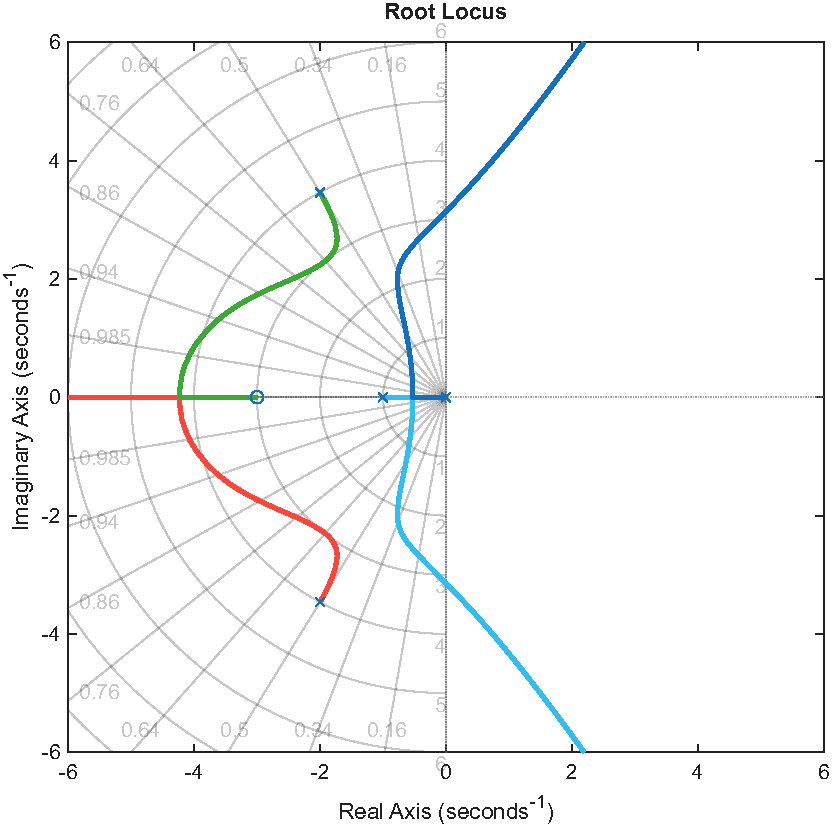
\includegraphics[width=0.8\linewidth]{rlocus_plot_test.pdf}
        \caption{Enter Caption}
        \label{fig:placeholder}
    \end{figure}
    \column{0.3\textwidth}
    Root Locus Plot of $$G(s) = \frac{K(s+3)}{s(s+1)(s^2+4s+16)}$$
    \lstinputlisting[
    frame=single,
    numbers=left,
    style=Matlab-Pyglike,
    basicstyle=\tiny, %or \small or \footnotesize etc.
    ]{matlab_files/rlocus_plot_test.m}
    \end{columns}
\end{frame}

\subsection{Diagram Example}
\begin{frame}{Basic Anatomy of Control System}
\tikzstyle{block} = [draw, fill=white, rectangle, 
    minimum height=3em, minimum width=6em]
\tikzstyle{sum} = [draw, fill=white, circle, node distance=1cm]
\tikzstyle{input} = [coordinate]
\tikzstyle{output} = [coordinate]
\tikzstyle{pinstyle} = [pin edge={to-,thin,black}]

% TO DO 
% Spreadout and build step by step
% Plant alone with input (u) and output relationship P(s)
% Insert Measurement
% Insert Reference
% Insert Error 
% Insert Controller and control law (u)
% Insert Disturbance
% Insert Sensor Noise/Bias

\begin{center}
\begin{tikzpicture}[auto, node distance=2cm,>=latex',
    block/.style={
            draw, 
            rectangle, 
            minimum height=3em, 
            minimum width=6em,
            % thick
        },
        sum/.style={
            draw, 
            circle, 
            node distance=1.5cm,
            path picture={
                \draw
                    (path picture bounding box.south west) -- (path picture bounding box.north east)
                    (path picture bounding box.north west) -- (path picture bounding box.south east);
            }
        },
        input/.style={coordinate},
        output/.style={coordinate},
        pinstyle/.style={pin edge={to-,thin,black}}
]

    \node [input, name=input] {};
    \node [sum, right of=input] (sum) {};
    \node [block, right of=sum] (controller) {Controller};
    \node [block, right of=controller, pin={[pinstyle]above:D},
            node distance=3cm] (system) {System};

    \draw [->] (controller) -- node[name=u] {$u$} (system);
    \node [output, right of=system] (output) {};
    \node [block, below of=u] (sensors) {Sensor};
    % \coordinate [below of=u] (sensors) {};

    \draw [->] (input) -- node {$r$} node[pos=0.9, above] {$+$} (sum);
    \draw [->] (sum) -- node {$e$} (controller);
    \draw [->] (system) -- node [name=y] {$y$}(output);
    %\draw [->] (y) |- (sensors);
    \draw [->] (y) |- (sensors);
    %\draw [->] (sensors) -| node[pos=0.99] {$-$} 
    \draw [->] (sensors) -| node [near end] {$y_m$} (sum) node[pos=0.95, right] {$-$} (sum);
        
    %\draw [->] 
\end{tikzpicture}    
\end{center}


\end{frame}

\begin{frame}{Frame Title}
    \begin{center}
\resizebox{0.9\textwidth}{!}{%
\begin{tikzpicture}[
    auto,
    node distance=2cm,
    >=latex',
    block/.style={
        draw, 
        rectangle, 
        minimum height=3em, 
        minimum width=6em,
        thick
    },
    sum/.style={
        draw, 
        circle, 
        node distance=1.5cm,
        path picture={
            \draw[thick]
                (path picture bounding box.south west) -- (path picture bounding box.north east)
                (path picture bounding box.north west) -- (path picture bounding box.south east);
        }
    },
    input/.style={coordinate},
    output/.style={coordinate},
    pinstyle/.style={pin edge={to-,thin,black}}
]

% Nodes
\node [input, name=input] {};
\node [sum, right of=input] (sum) {};
\node [block, right of=sum, node distance=5cm] (controller) 
    {$\dfrac{K(s+3)}{s(s+1)(s^2+4s+16)}$};
\node [output, right of=controller, node distance=5cm] (output) {};

% Arrows and labels
\draw [->, thick] (input) -- node[pos=0.3] {$R(s)$} node[pos=0.9, above] {$+$} (sum);
\draw [->, thick] (sum) -- node {$E(s)$} (controller);
\draw [->, thick] (controller) -- node [name=y] {} node[pos=0.95, above] {$C(s)$} (output);

% Feedback loop
\draw [->, thick] (y) |- ([yshift=-1.2cm]sum.south) -| node[pos=0.95, right] {$-$} (sum);

\end{tikzpicture}
}
\end{center}
\end{frame}

\begin{frame}{Root Locus Plot}
    Root Locus Plot of $$G(s) = \frac{K(s+3)}{s(s+1)(s^2+4s+16)}$$
    \pgfplotsset{compat=1.18}
% https://tex.stackexchange.com/questions/213183/root-locus-plots-using-latex
% Shared axis style applied to both plots
\pgfplotsset{
    splane axis/.style={
        axis lines=middle,
        xlabel={$\sigma$},
        ylabel={$j\omega$},
        xlabel style={anchor=north east},
        ylabel style={anchor=north west},
        grid=both,
        grid style={line width=.1pt, draw=gray!20},
        major grid style={line width=.2pt, draw=gray!50},
        tick label style={font=\footnotesize, fill=white, inner sep=1pt},
    }
}
%====================================================================
% Root locus data table
%====================================================================
\pgfplotstableread{
pr1 pi1 pr2 pi2 pr3 pi3 pr4 pi4 k
0	0	-2.000000000000000	3.464101615137757	-2.000000000000000	-3.464101615137757	-0.999999999999999	0	0
-0.119170902102986	0	-1.990414548948505	3.445845459189937	-1.990414548948505	-3.445845459189937	-0.899999999999999	0	0.566142857142857
-0.144071272308178	0	-1.988696638921510	3.442557894317898	-1.988696638921510	-3.442557894317898	-0.878535449848804	0	0.666869230414180
-0.175560546223051	0	-1.986668182067644	3.438669721408825	-1.986668182067644	-3.438669721408825	-0.851103089641657	0	0.785516526195408
-0.216544885337956	0	-1.984271989819692	3.434067741361256	-1.984271989819692	-3.434067741361256	-0.814911135022662	0	0.925273179185178
-0.272798311847314	0	-1.981439924310844	3.428615984667627	-1.981439924310844	-3.428615984667627	-0.764321839530997	0	1.089894900449838
-0.361029750860579	0	-1.978090635140101	3.422150522136338	-1.978090635140101	-3.422150522136338	-0.682788978859222	0	1.283805605467388
-0.508373684855238	0	-1.975610161293643	3.417349371885959	-1.975610161293643	-3.417349371885959	-0.540405992557477	0	1.426875214358039
-0.524414633535278	0	-1.975585357899669	3.417301307054558	-1.975585357899669	-3.417301307054558	-0.524414650665384	0	1.428303517875914
-0.524439446289494	0.016016580808805	-1.975560553710507	3.417253239568380	-1.975560553710507	-3.417253239568380	-0.524439446289494	-0.016016580808805	1.429731821393790
-0.525873237998957	0.122859463411328	-1.974126762001044	3.414472827120245	-1.974126762001044	-3.414472827120245	-0.525873237998957	-0.122859463411328	1.512216298974547
-0.530568548350443	0.252615864967427	-1.969431451649557	3.405341165289013	-1.969431451649557	-3.405341165289013	-0.530568548350443	-0.252615864967427	1.781265111435414
-0.536136014040702	0.349070247073217	-1.963863985959296	3.394459241691911	-1.963863985959296	-3.394459241691911	-0.536136014040702	-0.349070247073217	2.098182250362335
-0.542745753440391	0.437194505193579	-1.957254246559608	3.381460942134589	-1.957254246559608	-3.381460942134589	-0.542745753440391	-0.437194505193579	2.471484299261861
-0.550604355223086	0.523543081969902	-1.949395644776915	3.365889359023449	-1.949395644776915	-3.365889359023449	-0.550604355223086	-0.523543081969902	2.911203085643805
-0.559963980120549	0.611368338679338	-1.940036019879451	3.347167186132570	-1.940036019879451	-3.347167186132570	-0.559963980120549	-0.611368338679338	3.429155268513421
-0.571134134583971	0.702894818253275	-1.928865865416030	3.324553594232885	-1.928865865416030	-3.324553594232885	-0.571134134583971	-0.702894818253275	4.039259890030261
-0.584496847802434	0.800036845814749	-1.915503152197565	3.297079000647174	-1.915503152197565	-3.297079000647174	-0.584496847802434	-0.800036845814749	4.757912424968813
-0.600525743813230	0.904754835973144	-1.899474256186771	3.263441788309076	-1.899474256186771	-3.263441788309076	-0.600525743813230	-0.904754835973144	5.604425379893794
-0.619807880021483	1.019343595635013	-1.880192119978518	3.221835323259698	-1.880192119978518	-3.221835323259698	-0.619807880021483	-1.019343595635013	6.601547282367979
-0.643060126672927	1.146801111647280	-1.856939873327073	3.169637081748183	-1.856939873327073	-3.169637081748183	-0.643060126672927	-1.146801111647280	7.776074007102918
-0.671101622757162	1.291470420018752	-1.828898377242835	3.102797256761285	-1.828898377242835	-3.102797256761285	-0.671101622757162	-1.291470420018752	9.159568867353775
-0.704600608612204	1.460407086942255	-1.795399391387797	3.014487043040855	-1.795399391387797	-3.014487043040855	-0.704600608612204	-1.460407086942255	10.789210822731574
-0.742571850258799	1.666839349160141	-1.757428149741199	2.891645420585129	-1.757428149741199	-2.891645420585129	-0.742571850258799	-1.666839349160141	12.708793597506791
-0.771773969919931	1.939364113826105	-1.728226030080067	2.705784009431606	-1.728226030080067	-2.705784009431606	-0.771773969919931	-1.939364113826105	14.969902558928606
-0.771977918724984	1.983505603672081	-1.728022081275015	2.673521225009154	-1.728022081275015	-2.673521225009154	-0.771977918724984	-1.983505603672081	15.302827361821041
-0.770234792152947	2.028616490520570	-1.729765207847054	2.640087961358303	-1.729765207847054	-2.640087961358303	-0.770234792152947	-2.028616490520570	15.635752164713477
-0.759366978379084	2.120549311700363	-1.740633021620916	2.570936043634082	-1.740633021620916	-2.570936043634082	-0.759366978379084	-2.120549311700363	16.301601770498348
-0.737104460470923	2.211217369522394	-1.762895539529078	2.502327199560461	-1.762895539529078	-2.502327199560461	-0.737104460470923	-2.211217369522394	16.967451376283218
-0.704523458433218	2.295672664457096	-1.795476541566781	2.439257332153332	-1.795476541566781	-2.439257332153332	-0.704523458433218	-2.295672664457096	17.633300982068089
-0.658153895375609	2.383439387418269	-1.841846104624395	2.375874640973583	-1.841846104624395	-2.375874640973583	-0.658153895375609	-2.383439387418269	18.417616475196880
-0.608873879683611	2.458860635751211	-1.891126120316390	2.324024478842044	-1.891126120316390	-2.324024478842044	-0.608873879683611	-2.458860635751211	19.201931968325674
-0.513266570728435	2.582281225520941	-1.986733429271567	2.245523538940208	-1.986733429271567	-2.245523538940208	-0.513266570728435	-2.582281225520941	20.770562954583255
-0.322957963519513	2.795442021966142	-2.177042036480489	2.128219391094260	-2.177042036480489	-2.128219391094260	-0.322957963519513	-2.795442021966142	24.465996802812363
-0.147430930913150	2.982657191523247	-2.352569069086851	2.039625745588820	-2.352569069086851	-2.039625745588820	-0.147430930913150	-2.982657191523247	28.818910727845282
0.018272795789791	3.160759902665903	-2.518272795789791	1.962556650591351	-2.518272795789791	-1.962556650591351	0.018272795789791	-3.160759902665903	33.946281536505644
0.178211814111294	3.336936982915229	-2.678211814111295	1.889293398068907	-2.678211814111295	-1.889293398068907	0.178211814111294	-3.336936982915229	39.985898184634927
0.335166966831031	3.515045429608609	-2.835166966831030	1.815203639609671	-2.835166966831030	-1.815203639609671	0.335166966831031	-3.515045429608609	47.100064609803333
0.491112744045681	3.697531480288430	-2.991112744045681	1.736723388232170	-2.991112744045681	-1.736723388232170	0.491112744045681	-3.697531480288430	55.479961360480381
0.647532363087772	3.886153787725637	-3.147532363087772	1.650474742635168	-3.147532363087772	-1.650474742635168	0.647532363087772	-3.886153787725637	65.350783232678253
0.805602230282936	4.082303904022110	-3.305602230282939	1.552673788499769	-3.305602230282939	-1.552673788499769	0.805602230282936	-4.082303904022110	76.977790978899876
0.966301794945655	4.287166360958285	-3.466301794945658	1.438468590559546	-3.466301794945658	-1.438468590559546	0.966301794945655	-4.287166360958285	90.673439718288549
1.130481648081667	4.501806353208681	-3.630481648081666	1.300817170826556	-3.630481648081666	-1.300817170826556	1.130481648081667	-4.501806353208681	1.068057756113024e+02
1.298907552691661	4.727221490666744	-3.798907552691660	1.127934573685757	-3.798907552691660	-1.127934573685757	1.298907552691661	-4.727221490666744	1.258083264445853e+02
1.472290067265434	4.964374350883745	-3.972290067265436	0.895384679873214	-3.972290067265436	-0.895384679873214	1.472290067265434	-4.964374350883745	1.481917519178843e+02
1.564712988566932	5.092759203799709	-4.064712988566937	0.730768163050436	-4.064712988566937	-0.730768163050436	1.564712988566932	-5.092759203799709	1.613746593158005e+02
1.651305226168053	5.214214155261662	-4.151305226168052	0.521646215215871	-4.151305226168052	-0.521646215215871	1.651305226168053	-5.214214155261662	1.745575667137167e+02
1.694542412898369	5.275266449561593	-4.194542412898368	0.370437483044725	-4.194542412898368	-0.370437483044725	1.694542412898369	-5.275266449561593	1.814508974867525e+02
1.736507705341353	5.334774643783904	-4.236507705341348	0.060299653123896	-4.236507705341348	-0.060299653123896	1.736507705341353	-5.334774643783904	1.883442282597882e+02
1.737638433087004	5.336381434428870	-4.237638363094575	0	-4.237638503079436	0	1.737638433087004	-5.336381434428870	1.885327610208090e+02
1.738768276495925	5.337987144229602	-4.178476230721735	0	-4.299060322270116	0	1.738768276495925	-5.337987144229602	1.887212937818298e+02
1.836609484824339	5.477691992117714	-3.765826393891023	0	-4.907392575757649	0	1.836609484824339	-5.477691992117714	2.056143051328379e+02
2.028850881804324	5.755772069496501	-3.527758525536405	0	-5.529943238072248	0	2.028850881804324	-5.755772069496501	2.421965616912879e+02
2.228677645509119	6.049440457823748	-3.398890621198446	0	-6.058464669819791	0	2.228677645509119	-6.049440457823748	2.852874193611423e+02
2.436745041157560	6.359712216247428	-3.312934252769001	0	-6.560555829546119	0	2.436745041157560	-6.359712216247428	3.360448681739806e+02
2.653720988215452	6.687637469575558	-3.250718146177804	0	-7.056723830253099	0	2.653720988215452	-6.687637469575558	3.958329241399749e+02
2.880290810622407	7.034306806974349	-3.203626414344971	0	-7.556955206899846	0	2.880290810622407	-7.034306806974349	4.662582847481035e+02
3.117161373497740	7.400856252627554	-3.166962126963893	0	-8.067360620031582	0	3.117161373497740	-7.400856252627554	5.492135060987694e+02
3.365064788019096	7.788471981712956	-3.137859292516364	0	-8.592270283521820	0	3.365064788019096	-7.788471981712956	6.469278619773193e+02
3.624761817495059	8.198394905047323	-3.114434017322728	0	-9.135089617667409	0	3.624761817495059	-8.198394905047323	7.620272516154788e+02
3.897045084120899	8.631925212533034	-3.095380855460265	0	-9.698709312781544	0	3.897045084120899	-8.631925212533034	8.976047660550403e+02
4.182742152405179	9.090426943091014	-3.079759024685179	0	-10.285725280125185	0	4.182742152405179	-9.090426943091014	1.057303809459140e+03
4.482718548522557	9.575332633388802	-3.066869837592664	0	-10.898567259452468	0	4.482718548522557	-9.575332633388802	1.245416009108246e+03
4.797880762765560	10.088148087046482	-3.056182001075824	0	-11.539579524455297	0	4.797880762765560	-10.088148087046482	1.466996545237600e+03
5.129179273434703	10.630457298632480	-3.047283817096723	0	-12.211074729772678	0	5.129179273434703	-10.630457298632480	1.728000000000002e+03
1.214353410747289e+02	2.115168226286767e+02	-3.000005354824531	0	-2.448706767946333e+02	0	1.214353410747289e+02	-2.115168226286767e+02	1.456638062938572e+07
Inf	0	-3.000000000000000	0	Inf	0	Inf	0	Inf
}\mytable

%====================================================================
% Root locus, using the shared axis style
%====================================================================
\begin{center}
\resizebox{0.3\textwidth}{!}{%
\begin{tikzpicture}[
    start marker/.pic={\draw[thick] (-#1,-#1) -- (#1,#1) (#1,-#1)--(-#1,#1);}
]
\begin{axis}[
    splane axis,
    axis line style={opacity=0.4},          % more transparent axis lines
    tick style={opacity=0.4},                % match tick transparency
    xmin=-6, xmax=6,
    ymin=-6, ymax=6,
    xtick={-6,-4,-2,0,2,4,6},
    ytick={-6,-4,-2,0,2,4,6},
    clip mode=individual,                    % keep markers from being clipped
]
    % Shaded Stable Left-Half Plane (LHP) -- drawn first so curves sit on top
    \fill[green!10, opacity=0.2] (axis cs:-6,-6) rectangle (axis cs:0,6);

    % Shaded Unstable Right-Half Plane (RHP)
    \fill[red!10, opacity=0.2] (axis cs:0,-6) rectangle (axis cs:6,6);

\foreach\x in{1,...,4}{% Iterate over the four branch columns
  \addplot+[thick, mark=none] table[x=pr\x, y=pi\x] {\mytable}
    node[draw, circle, thick, inner sep=2pt] at (current plot end) {}% Ending marker
    pic at (current plot begin) {start marker=2pt};% Starting marker
}
\end{axis}
\end{tikzpicture}
} % for adjusting plot size
\end{center}
\end{frame}

% \begin{frame}{Electromechanical Diagram}
    % % Source - https://tex.stackexchange.com/a/514356
% Posted by nidhin, modified by community. See post 'Timeline' for change history
% Retrieved 2026-07-02, License - CC BY-SA 4.0
% https://www.overleaf.com/learn/latex/CircuiTikz_package

\documentclass[border=5mm]{standalone}
\usepackage{tikz}
\usepackage[american,siunitx]{circuitikz}
\usetikzlibrary{arrows,shapes,calc, positioning, patterns, decorations, decorations.markings,quotes}
\tikzset{rotarrow/.pic={
\draw[thin,->] (-0.2,-0.2)  to [out=-60,in=60, looseness=4] ++(0,0.4) node [above=1mm] {\tikzpictext};
},
}

\begin{document}
    \begin{tikzpicture}[damper/.style={thick,
            decorate,
            decoration={markings,  
                mark connection node=dmp,
                mark=at position 0.5 with 
                {
                    \node (dmp) [thick, inner sep=0pt, 
                    transform shape, 
                    rotate=-90, 
                    minimum width=15pt, 
                    minimum height=10pt, draw=none] {};
                    \draw [thick] ($(dmp.north east)+(4pt,0)$) -- 
                    (dmp.south east) -- (dmp.south west) -- 
                    ($(dmp.north west)+(4pt,0)$);
                    \draw [thick] ($(dmp.north)+(0,-8pt)$) -- 
                    ($(dmp.north)+(0,8pt)$);
        }}},]

        \draw (0,2) to[R=$R_a$,o-] ++(2,0) to[short,f=$i_a$] ++(0.1,0) to[L,cute inductor, l=$L_a$,]  ++(2,0)  to[short,  name=M1] ++(0,-2) to[short,-o] (0,0);
        \draw (M1) node[elmech,scale=0.7](M2){M};
        \path (0,2)node[below]{+} -- node[midway]{$E_a$} (0,0)node[above]{-};
        \draw[thick] (M2.east) -- pic[pic text={$T_m,\theta_m$}]{rotarrow} ++(1.5,0) -- +(0,0.5) node [anchor=south] {$N_1$} -- +(0,-0.5) coordinate (N1);

        \draw[thick] ([yshift=-2]N1) -- ++(0,-1.5) node [below] {$N_2$} ++(0,0.75) --  pic[xscale=-1,pic text={$\theta_L$}]{rotarrow} ++(1,0) node [cylinder, black, shape border rotate=180, draw,
        minimum height=2, minimum width=1, aspect=0.5,cylinder uses custom fill, cylinder end fill = black!70,anchor=west,xshift=-0.15cm, fill opacity=0.2,text opacity=1] (c) {Load Inertia};
        \draw [damper] (c.east) -- node[above=3mm] {$d_1$} ++(0:2)   node[draw, rectangle, minimum height=2cm, minimum width =0.5cm,anchor=west,preaction={fill=gray!10},pattern=north east lines,pattern=bricks]{};
    \end{tikzpicture}
\end{document}

% \end{frame}

\mode<beamer>{
  \begin{frame}
    This slide has intense animations and will ONLY appear in the presentation.
    It will be completely skipped in handout mode.
  \end{frame}
}

\end{document}
